\documentclass[12pt]{article}
\usepackage[spanish,mexico]{babel}
	\selectlanguage{spanish}
\usepackage{graphicx}
\usepackage{amsmath}
\usepackage{wrapfig}
\usepackage{float}
\usepackage{multicol}
\usepackage{geometry}
\usepackage{hyperref}
\usepackage[utf8]{inputenc}

\newgeometry{top=3cm}

\title{Actividad 5: Movimiento armónico simple: Péndulo}
\author{Ana Gabriela Carretas Talamante}
\date{16 de febrero de 2016}

\begin{document}
\maketitle
\section{Introducción}
Las matemáticas de los péndulos son generalmente complicadas. Se pueden asumir suposiciones simplificadas, entrando entonces en el caso del péndulo simple. Un péndulo simple es el modelo ideal de un péndulo real. Contempla las siguientes suposiciones:
\begin{itemize}
\item La cuerda con la que oscila el péndulo tiene una masa despreciable, es rígida y siempre se mantiene tensa.
\item El péndulo se maneja como masa puntual.
\item El movimiento se realiza en dos dimensiones, i.e., traza un arco al moverse.
\item El movimiento no pierde energía por la resistencia del aire o la fricción.
\item El campo gravitacional es uniforme.
\item El soporte que detiene al sistema no se mueve.
\end{itemize}
La ecuación diferencial que representa el movimiento de un péndulo simple es:
\begin{equation}
\label{1}
\frac{d^2\theta}{dt^2} + \frac{g}{l}\sin\theta=0
\end{equation}
donde $g$ es la aceleración causada por la gravedad, $l$ es la longitud del péndulo y $\theta$ es el desplazamiento angular. \\

La ecuación diferencial que describe el movimiento del péndulo simple no se resuelve sencillamente, y no hay solución analítica para ella. Pero si se añade una restricción en la amplitud de oscilación, resulta una forma de donde es fácil de obtener una solución. Si asumimos que $\theta \ll 1$, entonces $\sin\theta\approx\theta$, obteniendo así la ecuación del oscilador armónico:
\begin{equation}
\frac{d^2}{dt^2}+\frac{g}{l}\theta=0
\end{equation}
Si resolvemos con las siguientes condiciones iniciales, $\theta(0)=\theta_0, \frac{d\theta}{dt}(0)=0$:
\begin{equation}
\theta(t)=\theta_0\cos\left(\sqrt{\frac{g}{l}}t\right) \qquad \theta_0\ll1
\end{equation}
Este resulta en un movimiento armónico simple \cite{W}. \\

Resolver esta ecuación diferencial, como se mencionó anteriormente,  requiere el uso de diferentes métodos numéricos. Van desde los no tan precisos como el de Euler hasta los más famosos, como el de Runge-Kutta. En esta ocasión, utilizamos un método que viene integrado dentro las librerías de Python y que es sumamente sencillo de utilizar. \\

\begin{figure}[H]
\centering
\includegraphics[width=9cm]{0}
\caption{Péndulo simple \cite{P}.}
\end{figure}

El método \textit{scipy.integrate.odeint} nos ayuda a resolver ecuaciones diferenciales ordinarias al transformarlas en ecuaciones de primer orden por medio de un cambio de variable. De esta manera, podemos obtener una solución numérica para la ecuación. 

\pagebreak

\subparagraph*{Programa: Ecuación de un péndulo.}

Se presenta a continuación el código realizado, en donde se simularon diferentes casos en donde la amplitud y la velocidad angular inicial variaron. El código tiene la opción de resolver la ecuación para un péndulo simple o amortiguado, según se declare en las condiciones iniciales del programa. Se presentan también las gráficas arrojadas por el mismo, cada una refiriéndose a un caso distinto de condiciones iniciales.para poder simular diferentes casos en donde la amplitud y la velocidad angular inicial varían.

\begin{verbatim}
#Programa editado para múltiples casos
from scipy.integrate import odeint
import numpy as np
import matplotlib.pyplot as plt

#Definimos las constantes 
g=9.8             #Valor de la gravedad
l=0.5             #Longitud de la cuerda
b=0               #Amortiguamiento
c=g/l             #Frecuencia
theta=np.pi/2     #Angulo inicial
omega=1           #Velocidad inicial

#Definimos la función para el caso general; incluyendo el amortiguamiento
def pend(y, t, b, c):
     theta, omega = y
     dydt = [omega, -b*omega - c*np.sin(theta)]
     return dydt

#Definimos el intervalo de tiempo
t = np.linspace(0, 20, 1001)

#Evaluando la funcion
y0 = [theta, omega]
sol = odeint(pend, y0, t, args=(b, c))

#Para la grafica
plt.plot(t, sol[:, 0], 'm', label='theta(t)')
plt.plot(t, sol[:, 1], 'g', label='omega(t)')
plt.title("Simple pendulum")
plt.xlabel('Time')
plt.ylabel('Radians')
plt.legend(loc='best')
plt.grid()
plt.show()
\end{verbatim}

\begin{figure}[H]
\centering
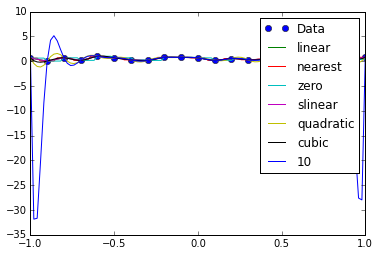
\includegraphics[width=7.5cm]{1}
\caption{Gráfica generada para las condiciones iniciales $\theta=\pi/2, \omega=1 \frac{rad}{s}$.}
\end{figure}

\begin{figure}[H]
\centering
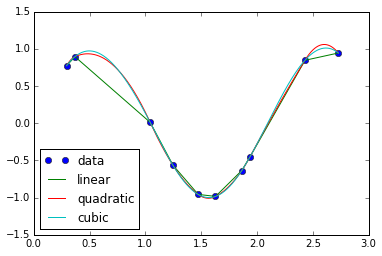
\includegraphics[width=7.5cm]{3}
\caption{Gráfica generada para las condiciones iniciales $\theta=\pi/3, \omega=5 \frac{rad}{s}$.}
\end{figure}

\begin{figure}[H]
\centering
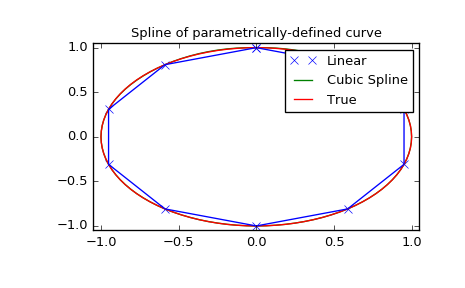
\includegraphics[width=7.5cm]{2}
\caption{Gráfica generada para las condiciones iniciales $\theta=0, \omega=0 \frac{rad}{s}$.}
\end{figure}

\begin{figure}[H]
\centering
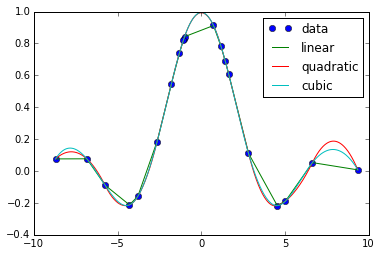
\includegraphics[width=7.5cm]{4}
\caption{Gráfica generada para las condiciones iniciales $\theta=\pi/3, \omega=5 \frac{rad}{s}, b=0.1$.}
\end{figure}

\begin{thebibliography}{6}

\bibitem{W}
Wikipedia,
\emph{Pendulum}. Recuperado el 16 de febrero de 2016 de \url{https://en.wikipedia.org/wiki/Pendulum\_(mathematics)}

\bibitem{P}
Chevtorno,
\emph{"Simple gravity pendulum" model assumes no friction or air resistance}. Recuperado el 16 de febrero de 2016 de \url{https://en.wikipedia.org/wiki/Pendulum#/media/File:Simple_gravity_pendulum.svg}

\bibitem{S1}
Scipy,
\emph{odeint}. \url{http://scipy.github.io/devdocs/generated/scipy.integrate.odeint.html}

\bibitem{FC}
Lizárraga, C.
\emph{Actividad 5 (2016-1)}. Recuperado el 16 de febrero de 2016 de \url{http://computacional1.pbworks.com/w/page/105233358/Actividad\%205\%20(2016-1)}

\end{thebibliography}

\end{document}

